

\section{Background}\label{sec:background}

In this section, we present the background of SSD internals (Section~\ref{sec:SSDInternals}) and search engine architectures (Section~\ref{sec:searchEngineArch}).

\subsection{Modern SSDs}\label{sec:SSDInternals}

\begin{figure}[htbp]
  \centering
  \begin{tabular}{ccc}
 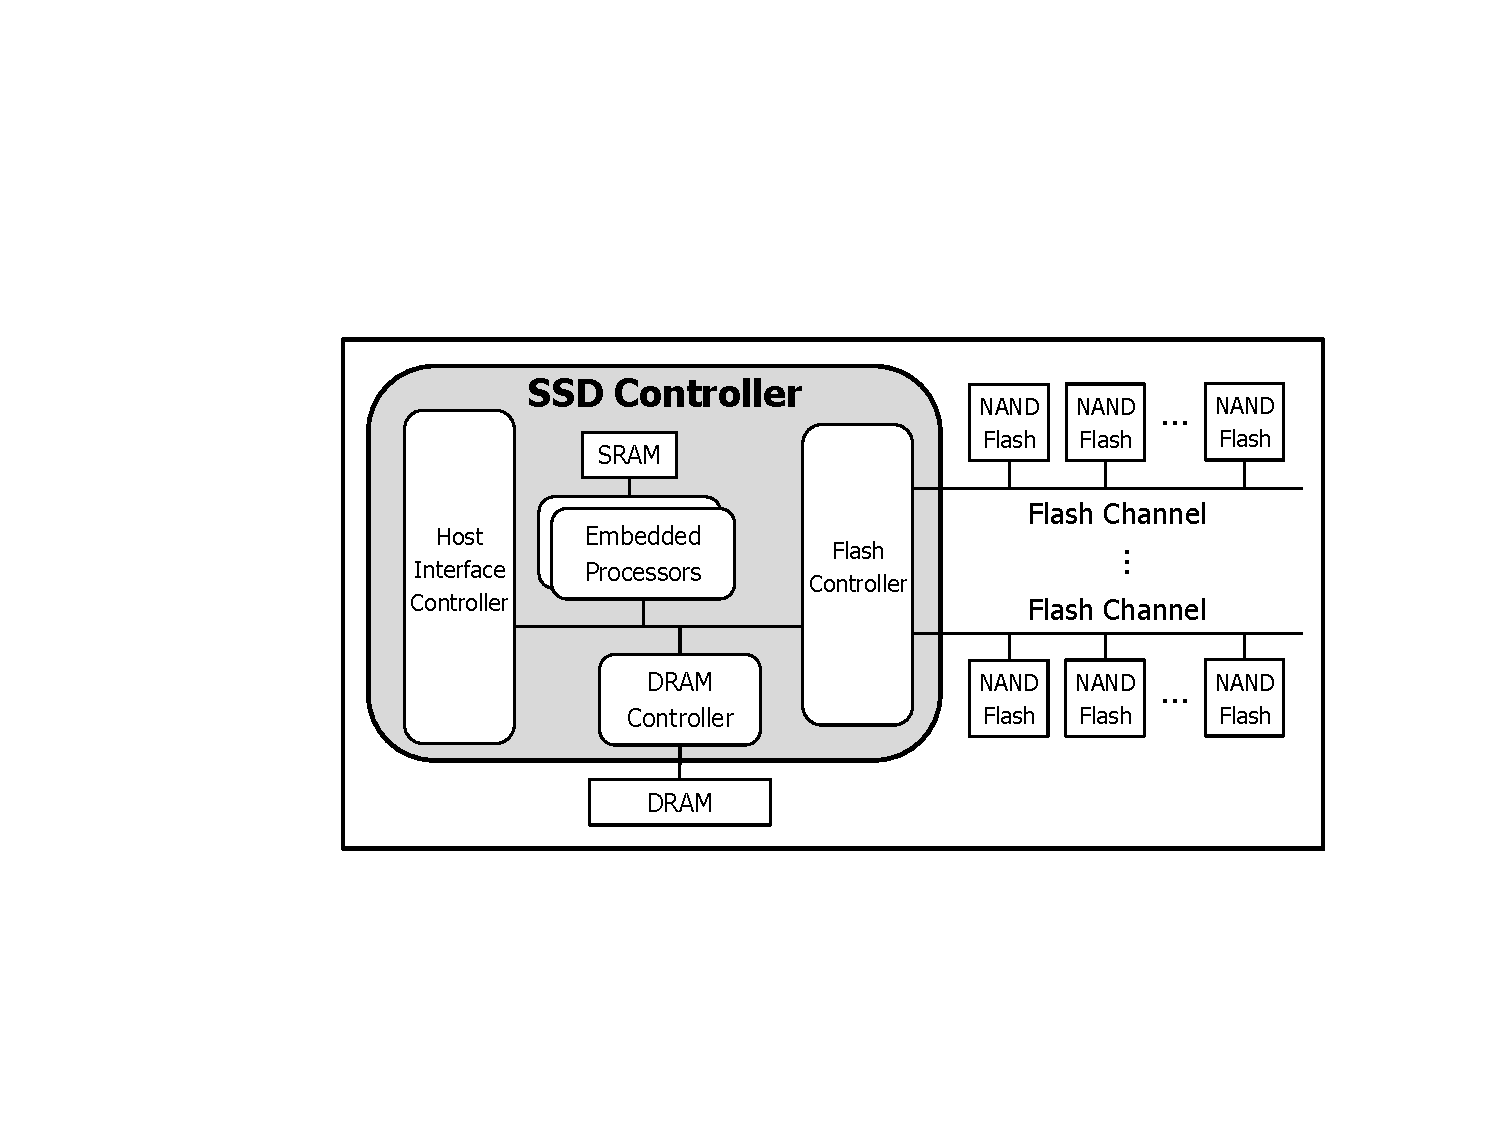
\includegraphics[width=1.0\columnwidth]{figures/SSDInternals.pdf}
\end{tabular}
  \caption{SSD internals}
  \label{fig:SSDInternals}
 \end{figure}

Figure~\ref{fig:SSDInternals} represents a typical modern SSD and its main components. In general, an SSD is largely composed of NAND flash memory array, SSD controller, and DRAM. The SSD controller subdivides into four main subcomponents such as host interface controller, embedded processors, DRAM controller, and flash memory controller.

Commands come from a user through the host interface and the most common interfaces, for instance, Serial ATA (SATA), Serial Attached SCSI (SAS), or PCI Express (PCIe), are implemented by the host interface controller.
The embedded processors in the SSD controller take the commands and pass them to the flash memory controller. They, more importantly, run SSD firmware codes for computation and execute Flash Translation Layer (FTL) for logical-to-physical address mapping. Typically, modern SSD is equipped with a low-powered 32-bit processor such as an ARM Cortex series processor and adopts multicore processors for better performance. Each processor can have a tightly coupled memory (e.g., SRAM) for the purpose of even faster access of frequently access data or codes. Each processor can access DRAM through the DRAM controller. For data transfer between flash memory and DRAM, the Flash Memory Controller (FMC) is adopted. This FMC runs Error Correction Codes (ECC) and supports Direct Memory Access (DMA) functionality.

The NAND flash memory package (also called chip) is persistent storage media and each package consists of one or more dies. The die is the smallest unit that can independently execute commands or report status. Each die contains one or more planes (usually one or two). Identical or concurrent operations can take place on each plane, although with some restrictions. Each plane subdivides into a number of blocks which are the smallest erase unit, and finally each block is composed of many pages (typically 64 or 128 pages)which are the smallest read/write unit.

An SSD is also equipped with a large size of DRAM for buffering data or storing meta data of the address mapping. All the flash channels share access to the DRAM. Thus, data transfer from the flash channels to the DRAM needs to be serialized.


\subsection{Web Search Engine}\label{sec:searchEngineArch}

\begin{figure}[htbp]
  \centering
  \begin{tabular}{ccc}
 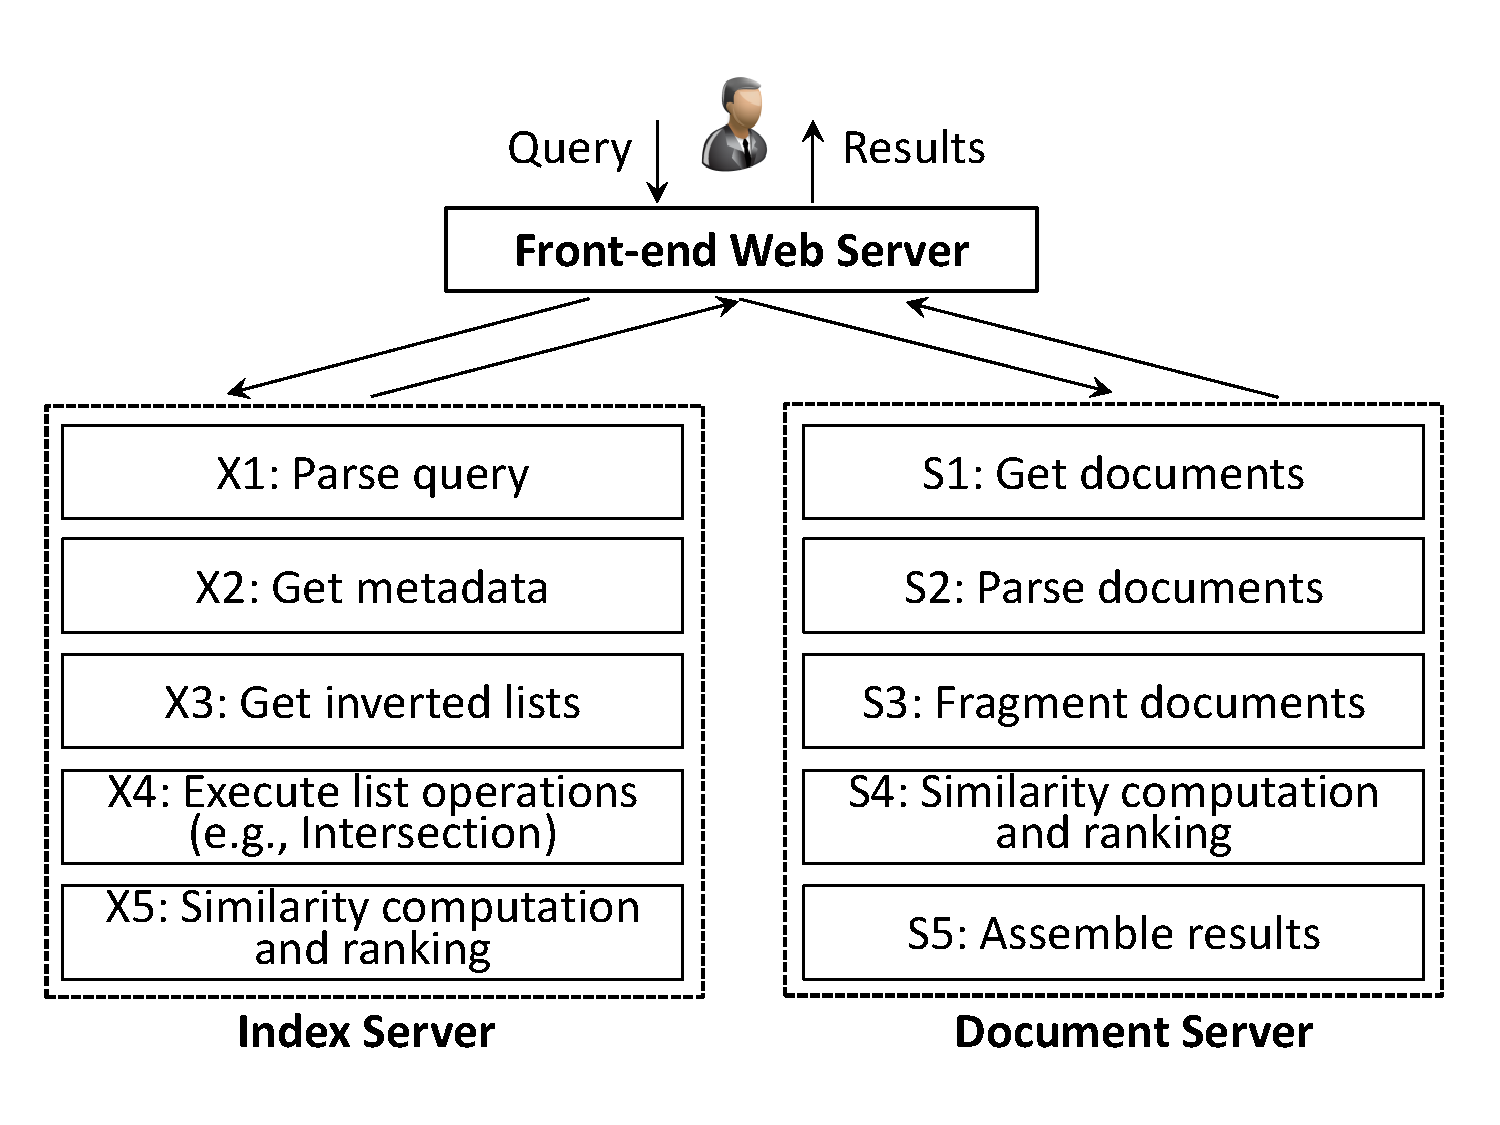
\includegraphics[width=1.0\columnwidth]{figures/searchEngineArch.pdf}
\end{tabular}
  \caption{Web search architecture}
  \label{fig:searchEngineArch}
 \end{figure}


Web search engine (WSE) is a complex large-scale software system with many components working together to answer user queries. Figure~\ref{fig:searchEngineArch} shows the system architecture of a typical web search engine, which includes three types of servers: front-end web server, index server and document server~\cite{Barroso2003WSP,BaezaYates07ICDE}.


\textbf{Front-end web server.} The front-end web server interacts with end users, mainly for receiving users' queries and returning the result pages. Upon receiving a query, depending on how the data is partitioned (e.g., term-based or document-based partitioning)~\cite{Dean2009}), it may or may not do some pre-processing, and forward the query to an index server.

\textbf{Index server.} The index server stores the inverted index~\cite{ZM06} to answer the query efficiently. It receives a query and return the top-$k$ most relevant document IDs, by going through several major steps (X1 to X5 in Figure~\ref{fig:searchEngineArch}).
\textit{Step X1}: parse the query into a parse tree (similar to the parse tree in database systems);
\textit{Step X2}: get the metadata for each inverted list. The metadata is consulted for loading the inverted list from disks. The metadata can include offset and length (in bytes) that the list is stored, may also include document frequency;
\textit{Step X3}: get the inverted list from disk to host memory, via the host I/O interface. Today, the inverted index is too big to fit into main memory~\cite{BaezaYates07ICDE,Risvik2013} and thus we assume the inverted index is stored on disks~\cite{Ruyue2010,Wang2013ISS};
\textit{Step X4}: do list operations depending on the query type. The basic operations include list intersection, union and difference~\cite{M08,GoogleAdv}.
\textit{Step X5}: for each qualified document, compute the similarity between the query and the document using an IR relevance model, e.g., the standard Okapi BM25 model~\cite{Robertson1994}. Then, return the top-$k$ most relevant document IDs to the web server for further processing.

\textbf{Document server.} The document server stores the actual documents (or web pages). It receives the query and a set of document IDs from the index server, then, generate query-specific snippets~\cite{Turpin2007FGR}. %which include a summarization of the document with query terms highlighted.
It also requires several query processing steps (S1 to S5 in Figure~\ref{fig:searchEngineArch}). \emph{Step S1} is to get the documents from disk, then, \emph{Step S2--S5} is to generate the query-specific snippets. We skip the details as our main focus is on index server.

This is the first work applying Smart SSD to search engine area. We mainly focus on the index server, and left the document server for future work. Based on our experience, on SSD-based search engines, query processing in the index server takes more time than in document server. 